\subsection{Representational analysis}\label{subsec:representation}

\subsubsection{Prediction error distribution analysis}\label{subsubsec:error_distribution_analysis}

To examine the prediction error distributions underlying the aggregate RMSE and Score metrics (Section~\ref{sec:results_ncmapss}), Fig.~\ref{fig:error_distribution_cmapss} and Fig.~\ref{fig:error_distribution_ncmapss} compare the distribution of prediction errors $(\hat{y}_i - y_i)$ for LBGN-RUL against a comparative baseline, binned into discrete error ranges whose widths match the score function's own asymmetric divisors (13 cycles for under-predictions, 10 cycles for over-predictions). For each dataset we show two transfers: LBGN-RUL's best-performing pair against its second-best comparative method, and its worst-performing pair against the single strongest baseline on that pair. The shaded region $[-13, 10]$ denotes the non-penalized interval in the NASA asymmetric scoring function.

On the best-performing pair on both datasets, LBGN-RUL concentrates a substantially larger share of predictions inside the non-penalized band than the comparative baseline (66.0\% vs.\ 50.0\% on CMAPSS F4$\to$F1 against DAST; 90.2\% vs.\ 31.3\% on N-CMAPSS D4$\to$D1 against CCDG), consistent with its RMSE advantage on these transfers (Tables~\ref{tab:cmapss_rmse}, \ref{tab:ncmapss_rmse}).

The worst-performing pairs are more differentiated, and we report both cases rather than the more favorable of the two. On CMAPSS F2$\to$F3, LBGN-RUL still attains the lowest RMSE among all compared methods despite a marginally lower in-region proportion than OCS-DANN (34.0\% vs.\ 37.0\%); Fig.~\ref{fig:error_distribution_cmapss} (right) shows this RMSE advantage is driven by fewer large-magnitude errors beyond $\pm40$ cycles rather than by a tighter concentration near zero, indicating that RMSE and in-region proportion capture different aspects of the error distribution and can diverge on individual transfers. On N-CMAPSS D1$\to$D3, by contrast, LBGN-RUL underperforms OCS-DANN across the distribution rather than in a single tail (33.9\% vs.\ 62.0\% in-region; Fig.~\ref{fig:error_distribution_ncmapss}, right), consistent with this being the one transfer pair, of the twelve evaluated, on which LBGN-RUL does not achieve the lowest RMSE.

\begin{figure}[!htbp]
\centering
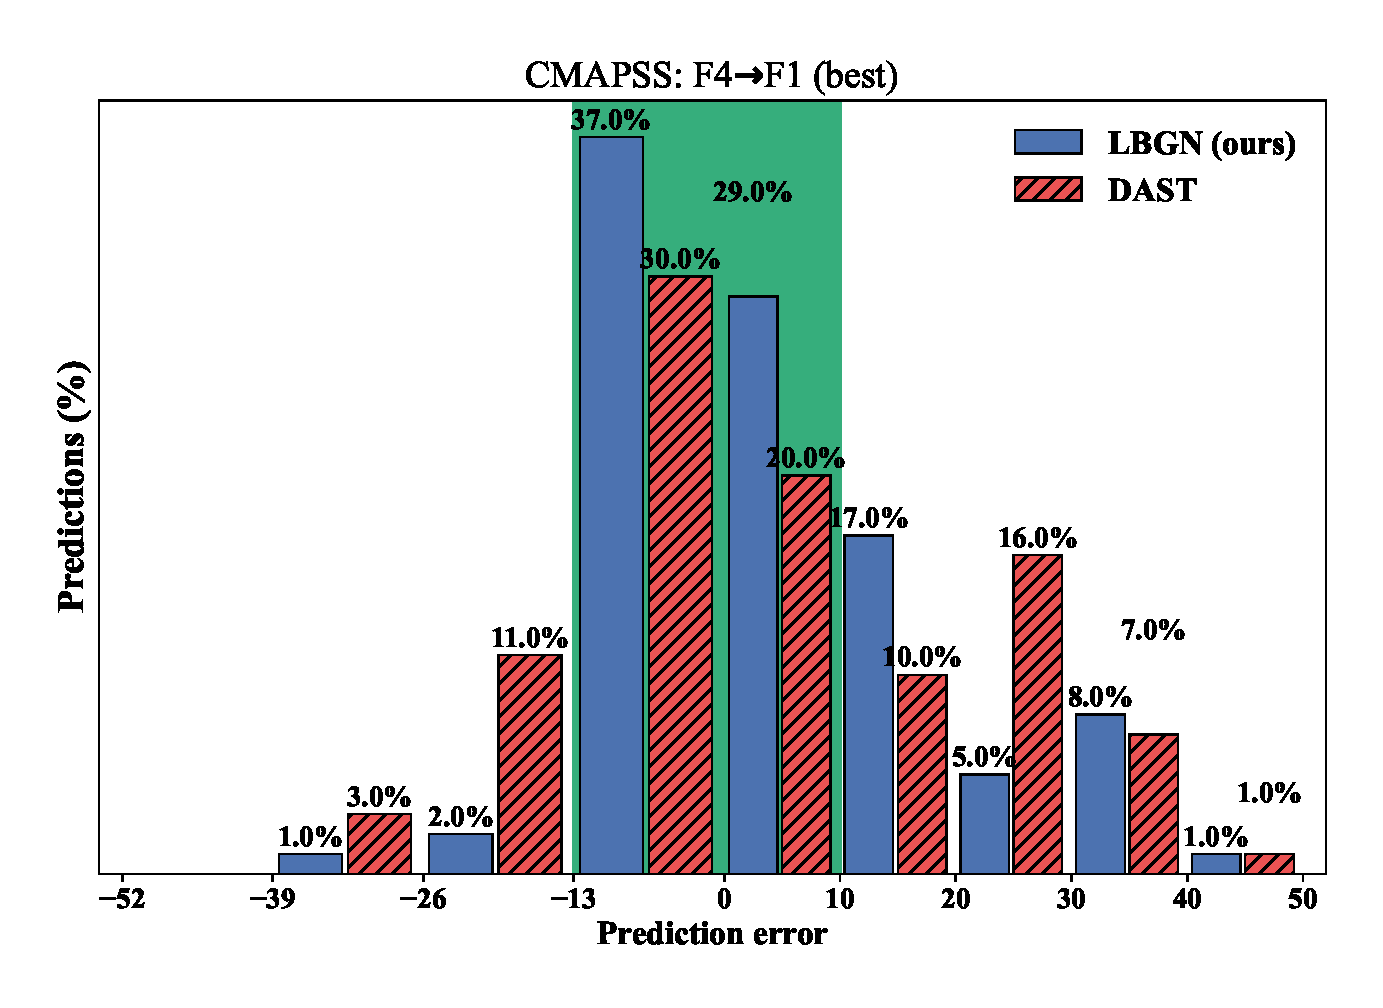
\includegraphics[width=0.48\linewidth]{fig_error_distribution_cmapss_best.eps}
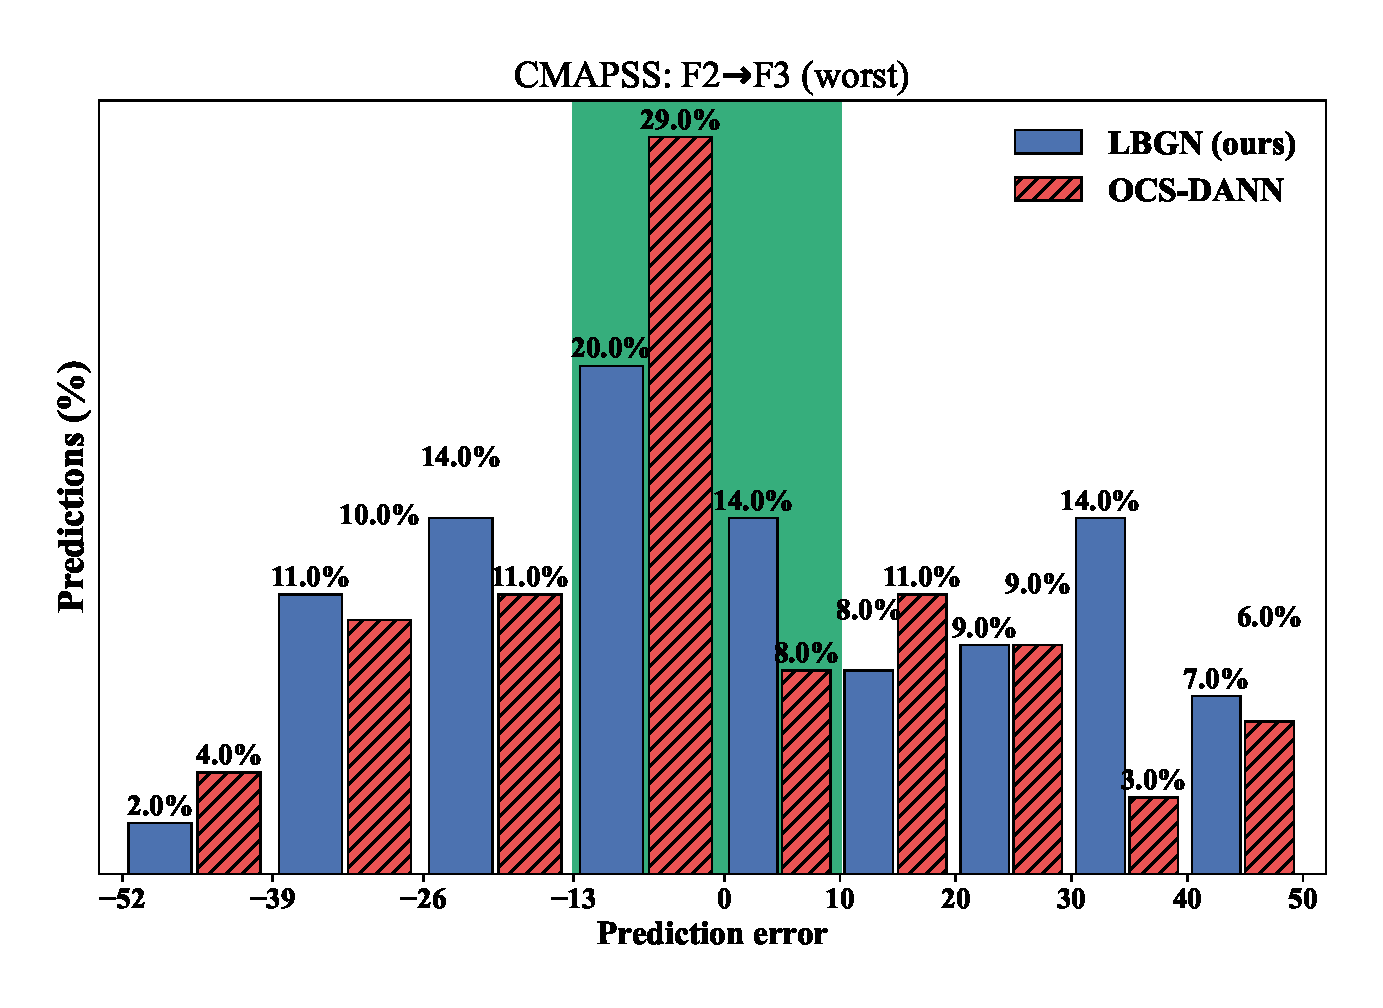
\includegraphics[width=0.48\linewidth]{fig_error_distribution_cmapss_worst.eps}
\caption{Distribution of prediction errors for LBGN-RUL versus a comparative baseline on CMAPSS: LBGN-RUL's best-performing transfer pair (F4$\to$F1, left, vs.\ DAST) and worst-performing transfer pair (F2$\to$F3, right, vs.\ OCS-DANN). The shaded region $[-13, 10]$ denotes the non-penalized error range under the scoring function.}
\label{fig:error_distribution_cmapss}
\end{figure}

\begin{figure}[!htbp]
\centering
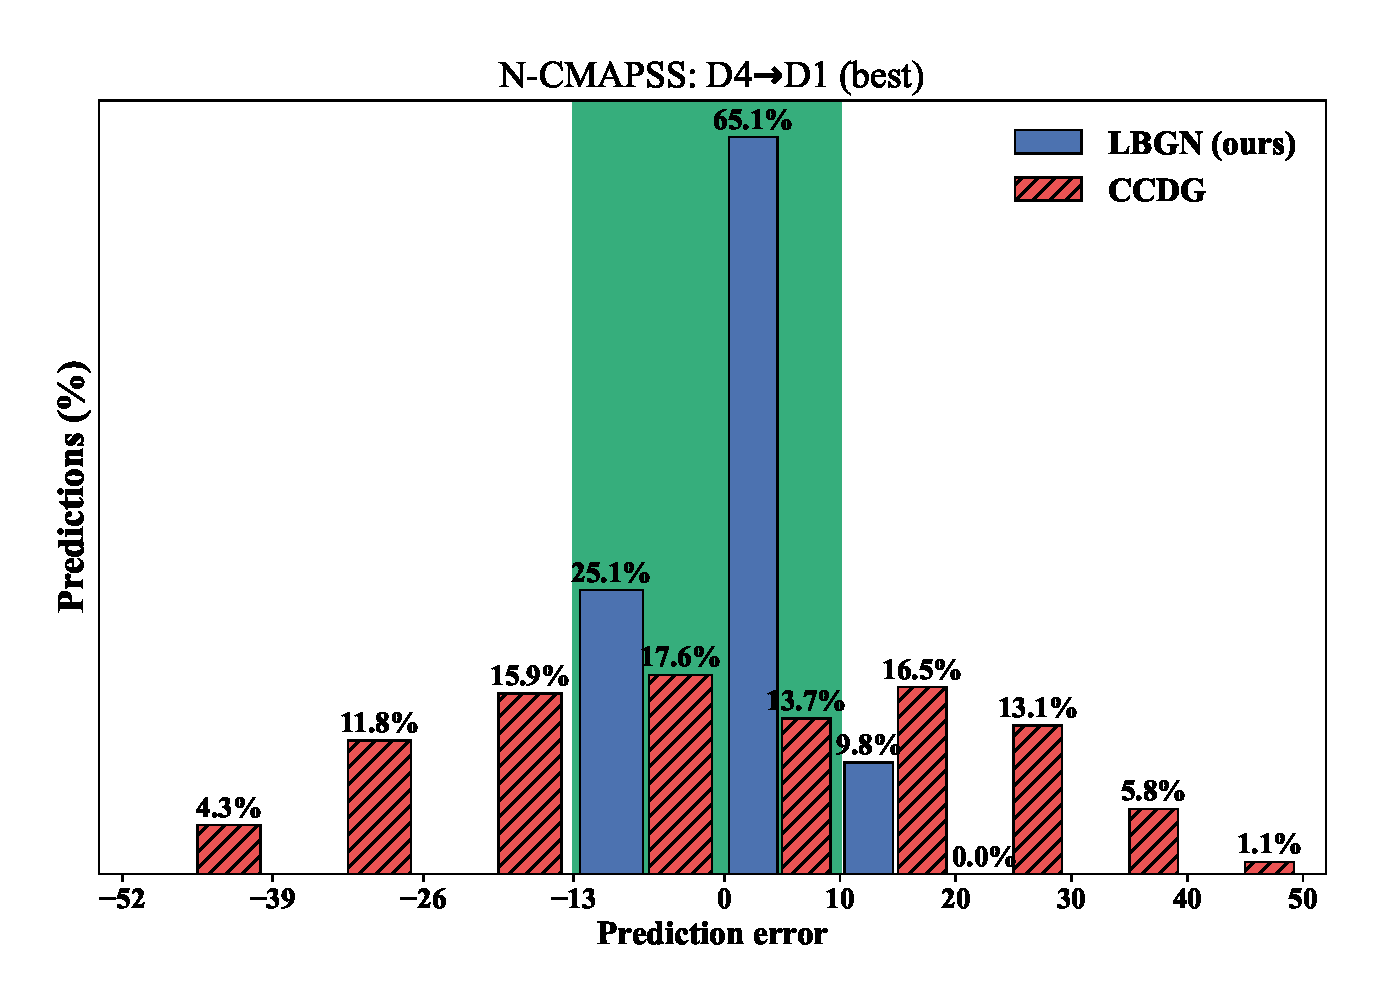
\includegraphics[width=0.48\linewidth]{fig_error_distribution_ncmapss_best.eps}
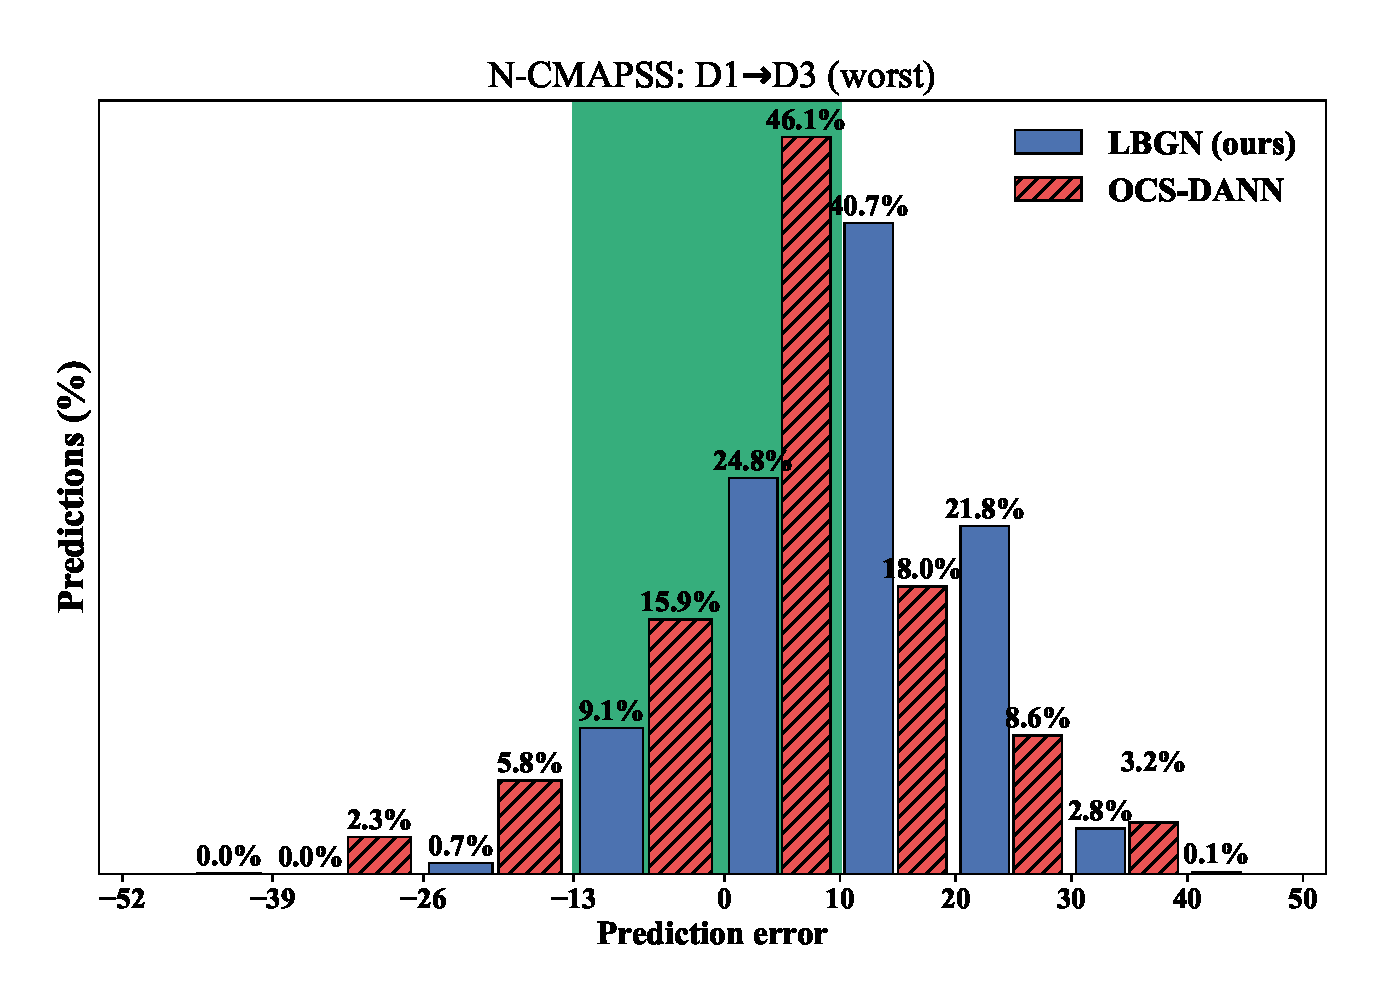
\includegraphics[width=0.48\linewidth]{fig_error_distribution_ncmapss_worst.eps}
\caption{Distribution of prediction errors for LBGN-RUL versus a comparative baseline on N-CMAPSS: LBGN-RUL's best-performing transfer pair (D4$\to$D1, left, vs.\ CCDG) and worst-performing transfer pair (D1$\to$D3, right, vs.\ OCS-DANN). The shaded region $[-13, 10]$ denotes the non-penalized error range under the scoring function.}
\label{fig:error_distribution_ncmapss}
\end{figure}
